\chapter{Theoretical Overview}

This chapter describes the physics backgrounds of the semileptonic VBS analysis.

\section{The Standard Model}

The Standard Model (SM) represents a description of the elementary particles and their interactions.
It is proved successful in explaining the results of existing experimental results so far, and predicting the later results.
All particles predicted by SM has been confirmed its existence, most recently the Higgs Boson found with ATLAS and CMS.
The SM predicts the existence of elementary particles which form the matter, which is fermion, classified into leptons and quarks.
The interactions of them are described by the gauge field mediated by the exchange of particles named bosons.
With these particles the model is describing three of the four known forces, which are the electromagnetic, the weak and the strong force. 
The theoretical description is given with the Quantum Field Theory (QFT) framework. The gauge invariance, which is the invariance of the local gauge transformation is the key of the framework. The underlying symmetry is described with the gauge group, SU(3)$_C \times$ SR(2)$_L \times$ U(1)$_Y$, which described in this section. These underlying structure of gauge theories can be described by Lie groups.

\subsection{Particle Content}
The 17 fundamental particles, which means particles with no substructure are considered in SM as the Figure~\ref{fig:SM} shows.
\begin{figure}[tbp]
\begin{center}
%\subfigure[]{
 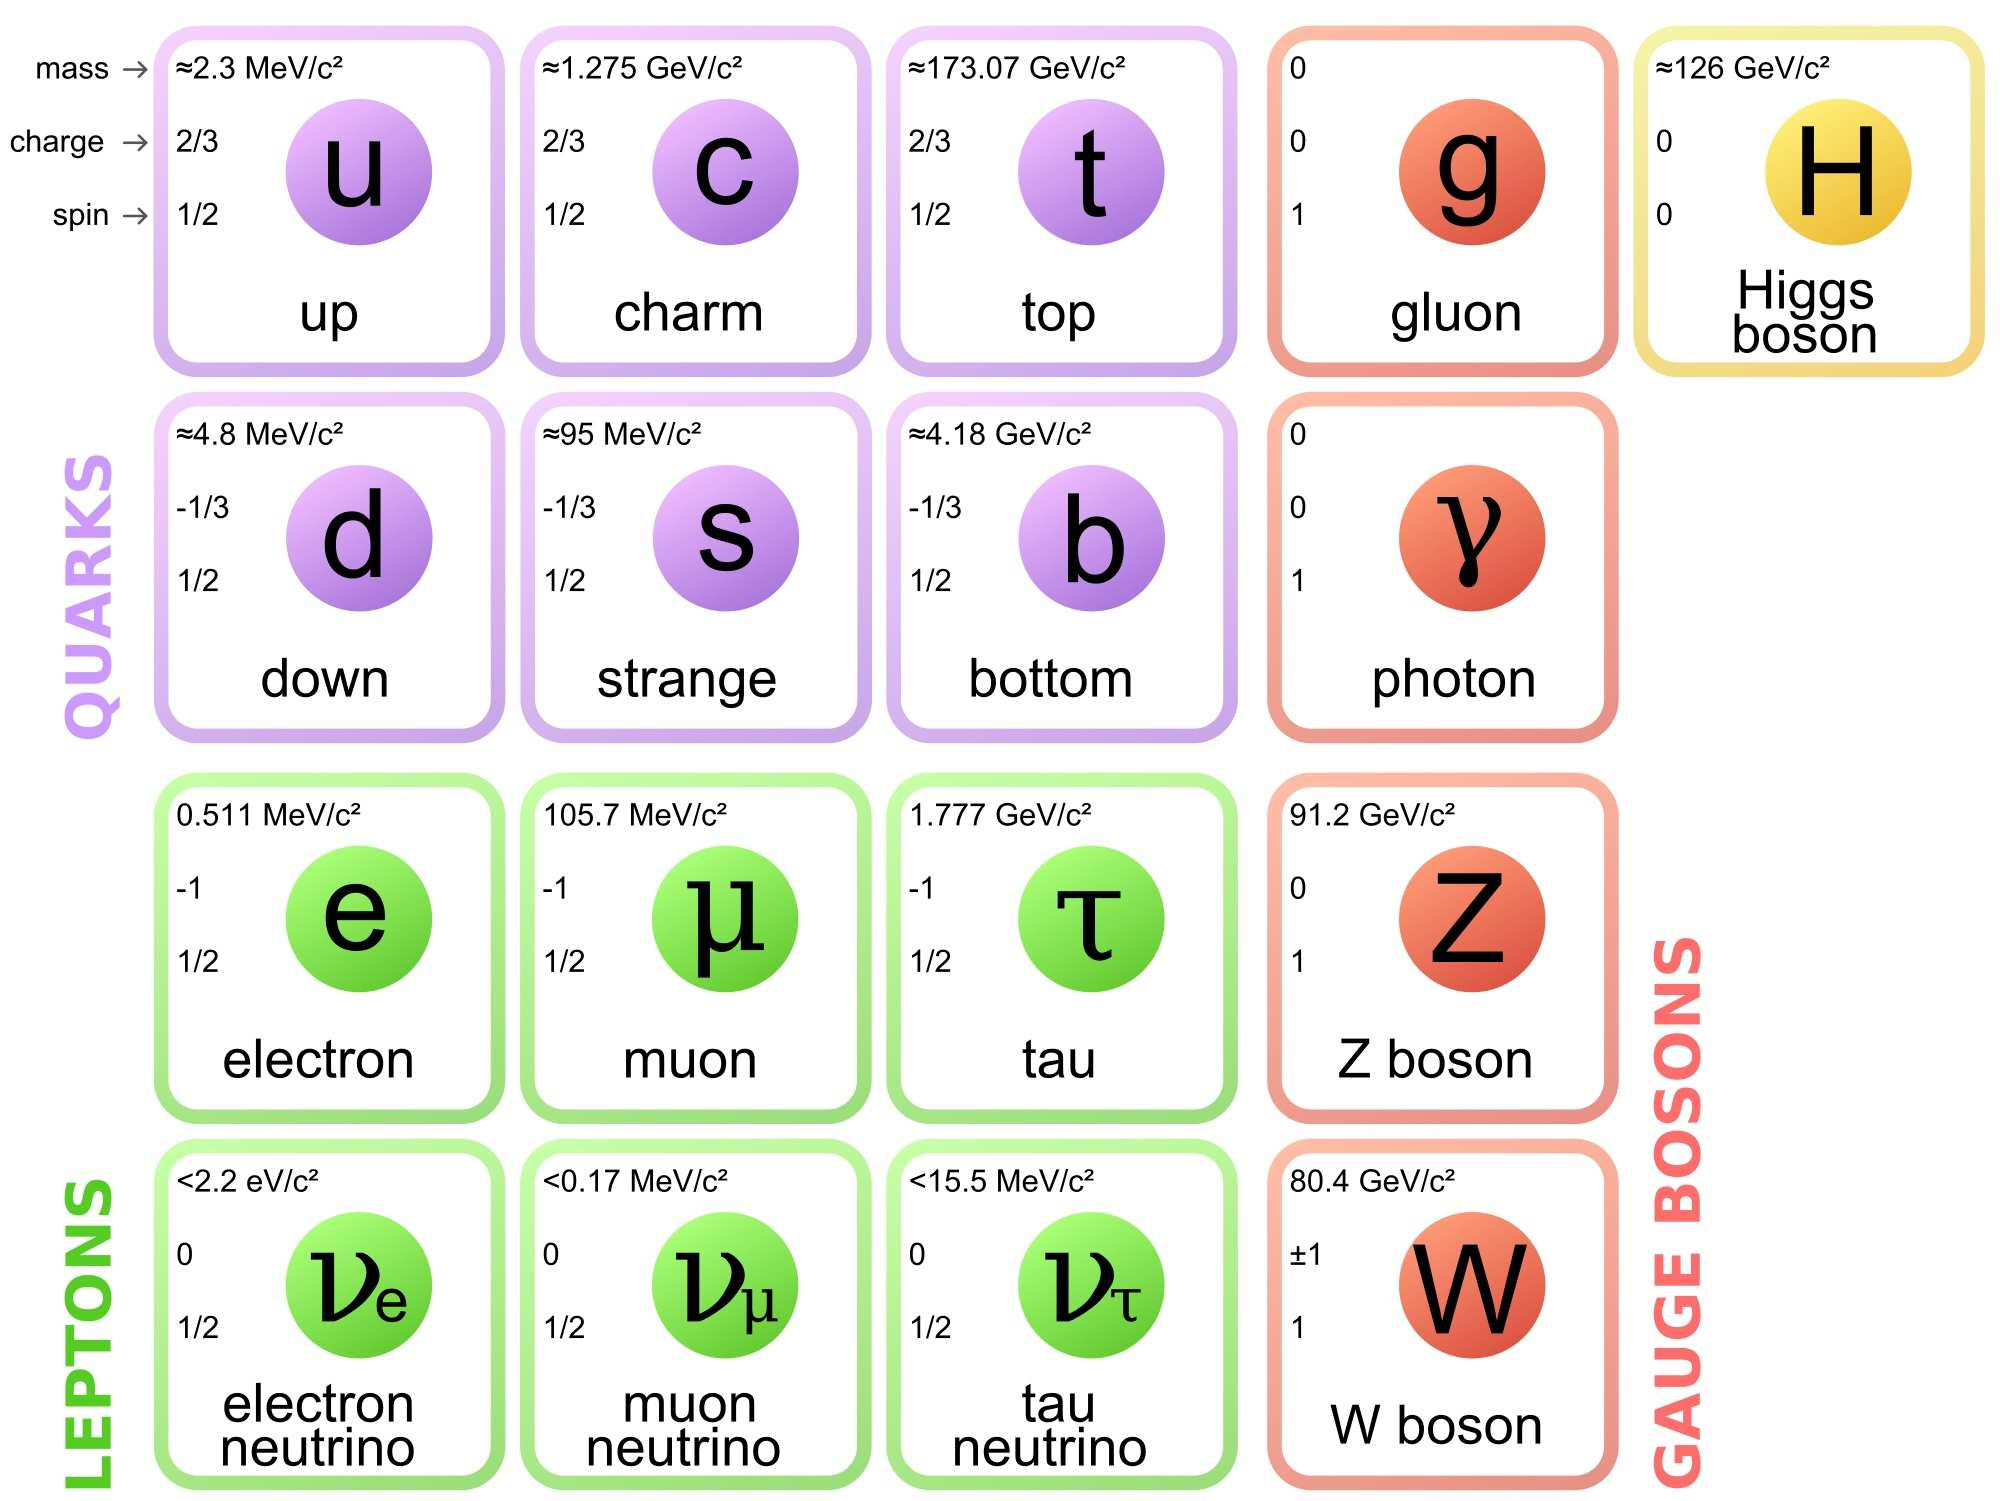
\includegraphics[width=0.85\textwidth,keepaspectratio]{figures/SM}
%}
\caption{
All particles exist in the SM %\ref{}
}
\label{fig:SM}
\end{center}
\end{figure}

There are two types of particles described in details below:
\begin{itemize}
    \item Fermion \\
    Fermions are the elementary particles with spin 1/2. There are three generations called flavors. The generations are classified only by the particle masses, increasing from first generation to the third generation. They are two types of fermions, quarks and leptons, each has 6 particles. Leptons do not act through the strong force, unlike the quarks.
    \item Boson \\
    Bosons are integer-spin particles and mediate the interaction of the fermions.
    The photons ($\gamma$) are mediator of the electromagnetic forces. The photons are massless and stable, and the electromagnetic force can be interact with infinite ranges. The photons interact with every particles with electric charges.\\
    The gluons (g) are the intermediate particles of the strong force. Also gluons are massless, and interact with the quarks and the gluons itselves.\\
    The W$^\pm$ and the Z bosons carry weak force. They are massive particles and interact with all particles carrying the weak charges. The W$^\pm$ can change the flavor of the quarks. \\
\end{itemize}

\subsection{SM Lagrangian}
\label{ch:Lagrangian}
The SM Lagrangian and its origin is to be shown here in this subsection. 
The Standard Model consists of several components as discribed in the follwing subsections. They are mathematically described as the Lagrangian density, $\mathcal{L}$, which is denoted as Lagrangian in the following.\\

\noindent\textbf{\sf{Quantum Electro Dynamis (QED)}} \\ 
The QED describes the dynamics of fermions and their electromagnatic interactions.

The free fermion with the spin 1/2 is described by the Lagrangian\\
\begin{equation}
\label{eqn:QED}
\mathcal{L}=i \bar{\psi} \gamma^{\mu} \partial_{\mu} \psi-m \bar{\psi} \psi
\end{equation}
The $\psi$ here is the spinor of the fermion field, $\gamma^{\mu}$  ($mu$ = 0,1,2,3) is the Dirac gamma 4$\times$4 matrix. $\partial_{\mu}$ = $\frac{\delta}{\delta x_{\mu}}$ are the partial derivatives, and the $\bar{\psi}=\psi^{\dagger} \gamma^{0}$.
For describing the equation of motion, the Dirac equation is given for $\psi$:
\begin{equation}
\left(i \gamma^{\mu} \partial_{\mu}-m\right) \psi=0
\end{equation}
The Lagrangian needs to be invariant with the "local" gauge transformation, i.e. the guage transformation parameter depends on x:
\begin{equation}
\psi(x) \rightarrow \psi^{\prime}(x)=e^{i \alpha(x)} \psi(x)
\end{equation}
where the local phase is given by $\alpha(x)$, depends on space and time. 
This transformation form the abelian unitary group U(1) with e$^i\alpha{x}$ can be written as the 1$\times$1 matrix with $U^{\dagger} U=1$.
The first term of the Lagrangian (\ref{eqn:QED}) is calculated and it is not invariant under this transformation:
\begin{equation}
\partial_{\mu} \psi \rightarrow \partial_{\mu} \psi^{\prime}=e^{i \alpha(x)} \partial_{\mu} \psi+i e^{i \alpha(x)} \psi \partial_{\mu} \alpha(x)
\end{equation}
The requirement of the invariance leads us to introduce an additional field A$_\mu$, transforming as:
\begin{equation}
A_{\mu} \rightarrow A_{\mu}^{\prime}=A_{\mu}+\frac{1}{e} \partial_{\mu} \alpha(x)
\end{equation}
where e is a coupling constant, which is elementary electric charge. 
and $\partial_{\mu}$ is replaced with the covariant derivative D$_\mu$:
\begin{equation}
D_{\mu}=\partial_{\mu}-i e A_{\mu}
\end{equation}
Then the derivative part can be replaced with:
\begin{equation}
D_{\mu} \psi \rightarrow D_{\mu}^{\prime} \psi^{\prime}=e^{i \alpha(x)} D_{\mu} \psi
\end{equation}
which leads the Lagrangian as:
\begin{equation}
\begin{aligned}
\mathcal{L} &=i \bar{\psi} \gamma^{\mu} D_{\mu} \psi-m \bar{\psi} \psi \\
&=\bar{\psi}\left(i \gamma^{\mu} \partial_{\mu}-m\right) \psi+e \bar{\psi} \gamma^{\mu} \psi A_{\mu}
\end{aligned}
\end{equation}
The Lagrangian now restore the invariance with the gauge field A$_\mu$. By using the strength tensor $F_{\mu \nu}=\partial_{\mu} A_{\nu}-\partial_{\nu} A_{\mu}$, the Lagrangian of QED is defined as:
\begin{equation}
\label{eqn:QEDLagrangian}
\mathcal{L}_{\mathrm{QED}}=i \bar{\psi} \gamma^{\mu} \partial_{\mu} \psi-m \bar{\psi} \psi+e \bar{\psi} \gamma^{\mu} \psi A_{\mu}-\frac{1}{4} F_{\mu \nu} F^{\mu \nu}
\end{equation}
The Lagrangian is invariant under the U(1)$_{EM}$ local gauge transformations of fields. The field A$_\mu$ is identified as photon, and the invariance forbids the introduction of a mass term of the A$_\mu$, of the form of $\frac{1}{2}m^2 A_\mu A^\mu$. The photon is requested to be massless, which agrees with all experiment results.
\\

\noindent\textbf{\sf{Quantum Chromo Dynamis (QCD))}} \\ 
The QCD describes the strong force interactions between quarks and gluons. The concept of the required invariance is similar to the QED, while an additional degree of freedom is introduced: the charge denoted as color, which is red (r), green(g), and blue(b). The Dirac spinor is replaced with vector of three spinors for quarks:
\begin{equation}
\psi=\left(\begin{array}{c}
\psi_{r} \\
\psi_{g} \\
\psi_{b}
\end{array}\right)
\end{equation}
The Lagrangian of QCD is described as:
\begin{equation}
\mathcal{L}_{\mathrm{QCD}}=i \bar{\psi} \gamma^{\mu} \partial_{\mu} \psi-m \bar{\psi} \psi-g_{s}\left(\bar{\psi} \gamma^{\mu} \frac{\lambda_{a}}{2} \psi\right) G_{\mu}^{a}-\frac{1}{4} G_{\mu \nu}^{a} G_{a}^{\mu \nu}
\end{equation}
with the gauge fields $G_{\mu}^{a}$ (a = 1,2,...,8) represents the gluons.
QED is an Abelian gauge theory since the underlying Lie group is the Abelian group U(1)$_{EW}$. For QCD, the underlying group is the non-Abelian group SU(3)$_C$, whose generators are T$_a$ = $\lambda_{a}/2$. $\lambda_{a}$ are callsed Gell-Mann matrices. They satisfy the commutator relation:
\begin{equation}
\left[\frac{\lambda_{a}}{2}, \frac{\lambda_{b}}{2}\right]=i f_{a b c} \frac{\lambda_{c}}{2}
\end{equation}
g$_s$ denotes the strong coupling constatnt, and $G_{a}^{\mu \nu}$ is the field strength tensor, written as:
\begin{equation}
G_{\mu \nu}^{a}=\partial_{\mu} G_{\nu}^{a}-\partial_{\nu} G_{\mu}^{a}-g_{s} f_{a b c} G_{\mu}^{b} G_{\nu}^{c}
\end{equation}
The non-Abelian group structure produces the last term of the field strength, which enables the gluons to interact with themselves differently from QED. Gluons are also requested to be massless from the gauge transformation of the fields.
%The whole Lagrangian for QCD??
\\ \\

\noindent\textbf{\sf{ElectroWeak Model}} \\
It is shown by experiments that the weak interaction only acts on left-handed fermions. In the electroweak model, the SU(2)$_L \times$ U(1)$_Y$ symmetry is conserved. Here the left-handed fermions are assigned to SU(2)$_L$ doublets with weak isospin I = 1/2, and gauge field W$^a_\mu$. The right-handed fermions are assigned to  U(1)$_Y$ singlets with weak isospin I = 0, and gauge field B$_\mu$.
%table of the quantum numbers
The left-handed doublets and right-handed singlet denote as $\chi_{L}$ and $\psi_{R}$ ,respectively. Specifically $\chi_{L}$ is written as 
$
\left(\begin{array}{c}
\nu_{L} \\
e_{L}
\end{array}\right)
$
for the leptons of the first generation, and $\psi_{R}$ is written as $(e_R)$.
For the quarks of the first generation, $\chi_{L}$ is 
$
\left(\begin{array}{c}
u_{L} \\
d_{L}
\end{array}\right)
$
and $\psi_{R}$ is $(u_R)$ and $(d_R)$.




These behave with local phase transformations as:
\begin{equation}
\begin{aligned}
\chi_{L}(x) \rightarrow \chi_{L}^{\prime}(x) &=e^{i \alpha_{a}(x) \tau_{a}} e^{i \beta(x) Y} \chi_{L} \\
\psi_{R}(x) \rightarrow \psi_{R}^{\prime}(x) &=e^{i \beta(x) Y} \psi_{R}
\end{aligned}
\end{equation}
where $\alpha_{a}(x)$ and $\beta(x)$ are the local phases, $\tau_{a}$ are the generators of SU(2)$_L$ with a = 1,2,3, and Y is the weak hypercharge operator of U(1)$_Y$. The covariant derivative is:
\begin{equation}
D_{\mu}=\partial_{\mu}+i g W_{\mu}^{a} \frac{\tau_{a}}{2}+i g^{\prime} B_{\mu} \frac{Y}{2}
\end{equation}
g here is the coupling constant of the SU(2)$_L$ gauge field written as $W_{\mu}^{a}$. $g^{\prime}$ is the coupling constant of the U(1)$_Y$ gauge field $B_{\mu}$.
The electroweak Lagrangian results in:
\begin{equation}
\mathcal{L}_{\mathrm{EW}}=i \overline{\chi_{L}^{i}} \gamma^{\mu} D_{\mu} \chi_{L}^{i}+i \overline{\psi_{R}^{i}} \gamma^{\mu} D_{\mu} \psi_{R}^{i}-\frac{1}{4} W_{\mu \nu}^{a} W_{a}^{\mu \nu}-\frac{1}{4} B_{\mu \nu} B^{\mu \nu}
\end{equation}
The field strength tensors are:
\begin{equation}
\begin{aligned}
W_{\mu \nu}^{a} &=\partial_{\mu} W_{\nu}^{a}-\partial_{\nu} W_{\mu}^{a}-g \epsilon_{a b c} W_{\mu}^{b} W_{\nu}^{c} \\
B_{\mu \nu} &=\partial_{\mu} B_{\nu}-\partial_{\nu} B_{\mu}
\end{aligned}
\end{equation}
where $\epsilon_{a b c}$ is an antisymmetric tensor, which is the structure constant of SU(2)$_L$. This term enables the $W_{a}^{\mu \nu}$ field to interact with themselves, while $B_{\mu}$ cannot self-interact.
The physical fields represents the W$^{\pm}$, Z bosons and photons are formed by linear combination of $W_{\mu \nu}^{a}$ and $B_{\mu \nu}$.
\begin{equation}
\begin{aligned}
W_{\mu}^{\pm} &=\frac{1}{\sqrt{2}}\left(W_{\mu}^{1} \mp i W_{\mu}^{2}\right) \\
Z_{\mu} &=\cos \theta_{W} W_{\mu}^{3}-\sin \theta_{W} B_{\mu} \\
A_{\mu} &=\sin \theta_{W} W_{\mu}^{3}+\cos \theta_{W} B_{\mu}
\end{aligned}
\end{equation}
where the $\theta_{W}$ = arctan ( g$^{\prime}$/g) represents the weak mixing angle, so called Weinberg angle. By rewriting the Lagrangian with physical fields and comparing the comparing the $A_{\mu}$ components with the QED Lagrangian (\ref{eqn:QEDLagrangian}), the relations between e and g, g$^{\prime}$ is obtained:
\begin{equation}
\begin{aligned}
e&=g \sin \theta_{W}=g^{\prime} \cos \theta_{W} \\
and \ \ Q&=I_{3}+\frac{Y}{2}
\end{aligned}
\end{equation}
The local gauge invariance forbid the introduction of the mass term of the 
The Lagrangian could include the mass terms of the bosons like $m^2_W W_\mu W^\mu$, while it is not invariant under $SU(2)_L \times U(1)_Y$ local transformations.
This statement that the local phase invariance in the electroweak model requests the fermions and bosons to be massless particles, is conflicted to the experimental results, where W$^{\pm}$ , Z bosons and fermions are found to be massive.
\\ \\
\noindent\textbf{\sf{Spontaneously Symmetry breaking}} \\ 
The conflict of the electroweak model of forbidding the mass of the fermions and boson can be solved by introducing a spontaneously symmetry breaking.
The mechanism is known as Brout-Englert-Higgs (BEH) mechanism or “Higgs mechanism” for short.

A complex scalar field, $\phi$, which is a weak isospin doublet is introduced as the Higgs field and has four degrees of freedom:
\begin{equation}
\label{eqn:higgsphi}
\phi=\left(\begin{array}{l}
\phi^{+} \\
\phi^{0}
\end{array}\right)=\frac{1}{\sqrt{2}}\left(\begin{array}{l}
\phi_{1}+i \phi_{2} \\
\phi_{3}+i \phi_{4}
\end{array}\right)
\end{equation}
The corresponding Lagrangian is written as:
\begin{equation}
\label{eqn:Higgs}
\mathcal{L}_{\text {Higgs }}=\left(D_{\mu} \phi\right)^{\dagger}\left(D^{\mu} \phi\right)-\mu^{2} \phi^{\dagger} \phi-\lambda\left(\phi^{\dagger} \phi\right)^{2}
\end{equation}
This is invariant under SU(2)$_l$ $\times$ U(1)$_Y$ phase transformation.
The potential of $\phi$ can be parametrize as:
\begin{equation}
V(\phi)=\mu^{2} \Phi^{\dagger} \phi+\lambda\left(\phi^{\dagger} \phi\right)^{2}
\end{equation}
where the $\lambda$ > 0. The value of the $\Phi$ at the vacuum is obtained by minimizing $V(\Phi)$. 
In case $-\mu^{2}>0$, the $V(\Phi)$ has its minimum value at 
\begin{equation}
\label{eqn:vacuum}
\phi_{0}&=\frac{1}{\sqrt{2}}\left(\begin{array}{l}
0 \\
v
\end{array}\right)
\end{equation}
where $v = \sqrt {-\mu^{2}/\lambda}$, while in case $-\mu^{2}<0, \phi_{0}=0$ gives the minimum of $V(\phi)$. 
The $v$ is called vacuum expectation value. In the former case, by assigning the ground state of the equation~\ref{eqn:vacuum} the local $SU(2)_L \times U(1)_Y$ symmetry of the vacuum is broken spontaneously. 
Three of the four degrees of freedom of the gauge field (\ref{eqn:higgsphi}) are absorbed by the $W^\pm$ and Z bosons, and the fourth generates the Higgs boson.

%The $\Phi(x)$ can be expanded near its minimum;
%\begin{equation}
%\phi=\frac{1}{\sqrt{2}} \exp \left(\frac{i}{2} \tau_{i} \chi^{\prime %i}(x)\right)\left(\begin{array}{c}
%0 \\
%v+h(x)
%\end{array}\right)
%\end{equation}
%where h(x) represents the Higgs Boson associated to the Higgs fields. The exponential containing  %$\chi^{\prime i}$ (x = 1,2,3) fields (GoldStone Boson) has three degrees of freedom. The local phase %invariance define a specific $\Phi$ as:
%\begin{equation}
%\phi=\frac{1}{\sqrt{2}}\left(\begin{array}{c}
%0 \\
%v+h(x)
%\end{array}\right)
%\end{equation}
%so compare to the equation ref{eqn:eqn:higgsphi}, $\phi_{1}=\phi_{2}=\phi_{4}=0$ and $\phi_{3} = v + %h(x)$. 

The field is parameterized as:
\begin{equation}
\phi(x)=\frac{e^{i \tau_{a} \theta_{a}(x) / v}}{\sqrt{2}}\left(\begin{array}{c}
0 \\
v+h(x)
\end{array}\right)
\end{equation}
where $\theta_{a}(x)$ (a = 1,2,3) and $h(x)$ are the real field, and  $h(x)$ represents the Higgs Boson which associated to the Higgs fields. The exponential term including $\theta_{a}(x)$ is defined to be specifical since local gauge transformation needs to be invariant;
\begin{equation}
\phi=\frac{1}{\sqrt{2}}\left(\begin{array}{c}
0 \\
v+h(x)
\end{array}\right)
\end{equation}
The specific gauge has chosen by defining the vacuum expectation value,which means the symmetry has broken spontaneously. 

The Lagrangian of Higgs (\ref{eqn:Higgs}) can be substituted and 
%%*****************************************
%\begin{equation}
%\left|\left(\partial_{\mu}+i g W_{\mu}^{a} \frac{\tau_{a}}{2}+i g^{\prime} B_{\mu} \frac{Y}{2} %\right) \frac{1}{\sqrt{2}}\left(\begin{array}{l}
%0 \\
%v
%\end{array}\right) \right| -\mu^{2} \Phi^{\dagger} \Phi-\lambda\left(\Phi^{\dagger} %\Phi\right)^{2}
%\end{equation}
%%*****************************************
the term represents the mass terms and its relations are written as:
\begin{equation}
\begin{aligned}
\left|\left(i g \frac{\tau_{a}}{2} W_{\mu}^{a}+i g^{\prime} \frac{Y}{2} B_{\mu}\right) \phi_{0}\right|=&\left(\frac{1}{2} v g\right)^{2} W_{\mu}^{+} W^{\mu-} \\
&+\left(\frac{1}{2} v g\right)^{2} \frac{1}{2 \cos ^{2} \theta_{W}} Z_{\mu} Z^{\mu} \\
&+0 \cdot A_{\mu} A^{\mu}
\end{aligned}
\end{equation}
%%Calculate this!
%which the mass terms of the vector bosons can be written:
%\begin{equation}
%\begin{aligned}
%m_{W}&=\frac{1}{2} vg \\
%m_{Z}&=\frac{m_{W}}{\cos \theta_{W}} \\
%m_{\gamma}&=0
%\end{aligned}
%\end{equation}
The mass terms for the $W_\pm$ and Z bosons naturally obtained through the symmetry breaking of SU(2)$_L$. :
\begin{equation}
\begin{aligned}
m_{\gamma} &=m_{A}=0 \\
m_{Z} &=\frac{v}{2} \sqrt{g^{2}+g^{\prime 2}} \\
m_{W} &=\frac{v}{2} g
\end{aligned}
\end{equation}

%The $A_\mu$ does not acquire the mass term, as the photons are remained to be massless.
%There is a term $-\mu_{\phi}^{2} h^{2}=\lambda v^{2} h^{2}$ and from this term the Higgs boson %gains mass itself, which leads to the Higgs boson mass 
%\begin{equation}
%m_{H}=\sqrt{-2 \mu^{2}}=\sqrt{2 \lambda} v
%\end{equation}
%The parameter $\lambda$ is a free parameter in the theory, so it cannot be predicted by the SM.
%The vacuum expectation value is is determined by the measurements of the Fermi constant $G_F$, %which is to be:
%%put reference here (measurement of the Fermi coupling) 
%\begin{equation}
%v=\frac{2 m_{W}}{g}=\frac{1}{\sqrt{2} G_{F}} \simeq 246.22 \mathrm{GeV}
%\end{equation}

The fermion mass term is also not invariant under the local phase transformations of SU(2)$_L$. It is also generated with the Higgs mechanism, using their coupling to the Higgs boson. The newly introduced coupling $g_f$ is called Yukawa coupling.

For the down type fermions, the same Higgs field $\phi$ is used, while for the up type fermions, the charge conjugate of the Higgs field $\phi^C$ is used:
\begin{equation}
\phi^{c}=i \tau_{2} \phi^{*}=\left(\begin{array}{c}
\phi^{0 *} \\
-\phi^{+*}
\end{array}\right)
\end{equation}
For the quarks, the additional Lagrangian can be described as follows:
\begin{equation}
\mathcal{L}_{q}=\left[-g_{d}\left(\bar{\psi}_{L}^{d} \phi \psi_{R}^{d}\right)+\text { h.c. }\right]+\left[-g_{u}\left(\bar{\psi}_{L}^{u} \phi^{c} \psi_{R}^{u}\right)+\text { h.c. }\right]
\end{equation}
These are local gauge invariant before the symmetry breaking. After the symmetry breaking, $\phi^C$ can be written as:
\begin{equation}
\phi^{c} 
%\rightarrow 
=\frac{1}{\sqrt{2}}\left(\begin{array}{c}
v+h \\
0
\end{array}\right)
\end{equation}
Then the additional Lagrangian substituted into:
\begin{equation}
\mathcal{L}_{q}=-\frac{1}{\sqrt{2}} g_{d} v \bar{d}_{L} d_{R}\left(1+\frac{h}{v}\right)-\frac{1}{\sqrt{2}} g_{u} v \bar{u}_{L} u_{R}\left(1+\frac{h}{v}\right)
\end{equation}
In case of leptons the original additional Lagrangian is:
\begin{equation}
\mathcal{L}_{e}=\left[-g_{e}\left(\bar{\psi}_{L}^{e} \phi \psi_{R}^{e}\right)+\text { h.c. }\right]
\end{equation}
then after the symmetry breaking:
\begin{equation}
\mathcal{L}_{e}=-\frac{1}{\sqrt{2}} g_{e} v \bar{e}_{L} e_{R}\left(1+\frac{h}{v}\right)
\end{equation}

The mass of the fermions is to be obtained as:
\begin{equation}
m_{f}=\frac{1}{\sqrt{2}} g_{f} v
\end{equation}

When summarizing the quarks and leptons, Lagrangian of the Yukawa couplings can be written as:
\begin{equation}
\mathcal{L}_{\text {Yukawa }}=-g_{l}^{i j} \bar{\Psi}_{L}^{i} \phi l_{R}^{j}-g_{d}^{i j} \bar{\Psi}_{L}^{i} \phi d_{R}^{j}-g_{u}^{i j} \bar{\Psi}_{L}^{i} \phi^{C} u_{R}^{j}+\text { h.c. }
%?? is this correct ??
\end{equation}

At last, the Standard Model Lagrangian is described as 
\begin{equation}
\mathcal{L}_{\mathrm{SM}}=\mathcal{L}_{\mathrm{QCD}}+\mathcal{L}_{\mathrm{EW}}+\mathcal{L}_{\text {Higgs }}+\mathcal{L}_{\text {Yukawa}}
\end{equation}
This Lagrangian is invariant under local transformations of SU(3) $\times$ SU(2)$_L$ $\times$ U(1)$_Y$, while the vacuum is breaking the symmetry and not invariant. \\

The coupling constats appeared in the Lagrangian are determined by the measurement from experiments. The measured valued is summarized in the Table~ref{tab:constants}.  

\begin{tabular}{|l|l|}
\hline Coupling constants & Measured Value \\
\hline & $y_{u}=10^{-5}, y_{c}=7 \times 10^{-5}, y_{t}=1,$, \\
Yukawa Couplings & $y_{d}=3 \times 10^{-5}, y_{s}=5 \times 10^{-4}, y_{b}=0.03$ \\
& $y_{e}=3 \times 10^{-6}, y_{\mu}=6 \times 10^{-4}, y_{\tau}=0.01$ \\
Fine Structure Constant & $\alpha=1 / 127$ \\
Strong Coupling Constant & $\alpha_{s}=0.12$ \\
Weinberg Angle & $s_{W}^{2}=0.23$ \\
Higgs Self Coupling Constant & $\lambda=0.1$ \\
PMNS matrix (parametric representation) & $\theta_{12}=34, \theta_{13}=8.5, \theta_{23}=247, \delta_{C P}=200$ \\
CKM matrix (parametric representation) & $\theta_{12}=13.0, \theta_{13}=0.2, \theta_{23}=2.4, \delta_{13}=1.2$ \\
\hline
\label{tab:constants}
\end{tabular}

\section{Phenomenology of proton-proton collisions}
\textcoler{red}{This section needs to be added}

\section{Vector Boson Scattering}
The scattering of two electroweak gauge bosons can probe the structure of the electroweak symmetry breaking (EWSM) mechanism directly. 
Electroweak gauge boson scattering, or Vector Boson Scattering (VBS) is therefore one of the key process to be investigate in LHC experiment.
The Vector Boson indicates W,Z,$\gamma$ here, which are fundamental electroweak bosons. Though the massive vector bosons, which is W and Z are only sensitive to the mechanism of the  EWSM, $\gamma$ is also included since it is impossible to fully separate the $\gamma$ and Z contributions experimentally. 
%<- need this??
\subsection{Electroweak gauge boson scattering and the Higgs boson}
As described in Chapter~\ref{ch:Lagrangian}, the spontaneously symmetry breaking of the local gauge invariance produces three degrees of freedom, which is the GoldStone Bosons and then they are eaten up by the introducing of the Higgs Boson. They correspond to the longitudinal, massive weak gauge bosons. Measuring the VBS channels provides information of the other three degrees of freedom than Higgs field. The typical Feynman diagram of VBS is shown in Figure~\ref{fig:VBS}.
%%Correct explanation here????

\begin{figure}[tbp]
\begin{center}
%\subfigure[]{
 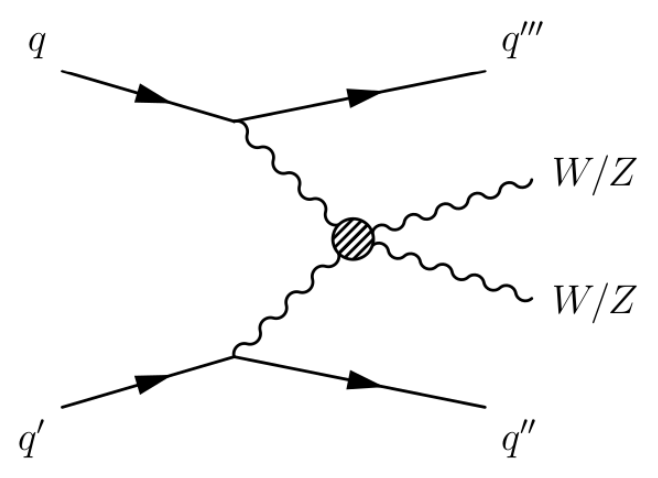
\includegraphics[width=0.50\textwidth,keepaspectratio]{figures/VBS}
%}
\caption{
The Feynman diagram of the VBS. The circle includes any connected diagrams with the external lines at leading order.%, as shown in the Figure\ref{}.
}
\label{fig:VBS}
\end{center}
\end{figure}

\begin{figure}[tbp]
\begin{center}
\subfigure{
 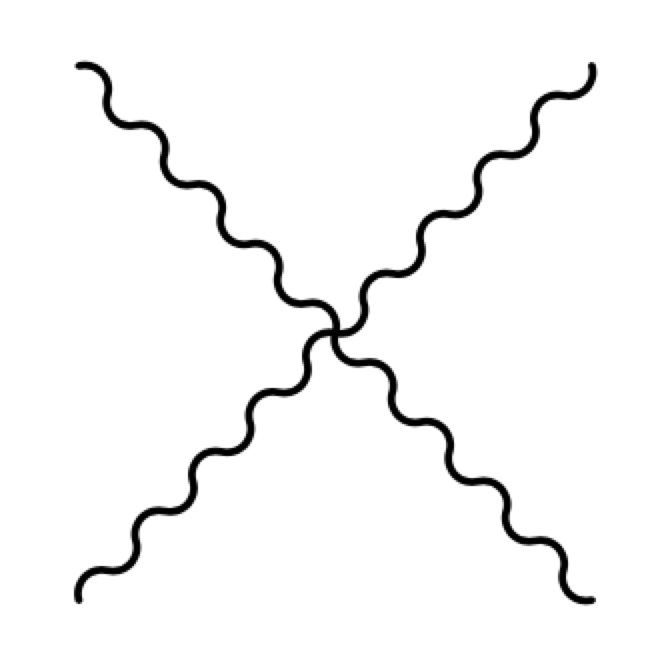
\includegraphics[width=0.20\textwidth,keepaspectratio]{figures/VBS1}
}
\subfigure{
 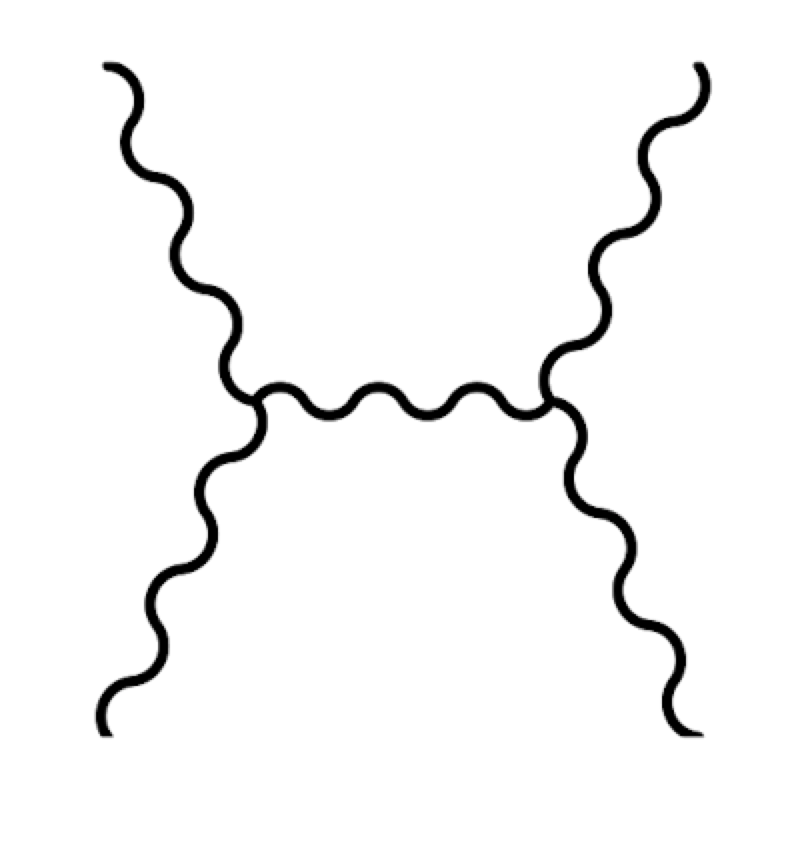
\includegraphics[width=0.19\textwidth,keepaspectratio]{figures/VBS2}
}
\subfigure{
 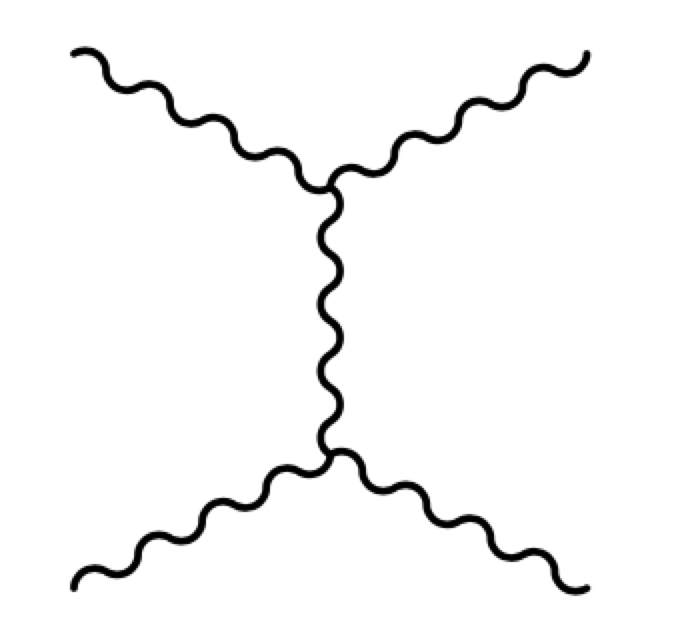
\includegraphics[width=0.21\textwidth,keepaspectratio]{figures/VBS3}
}
\subfigure{
 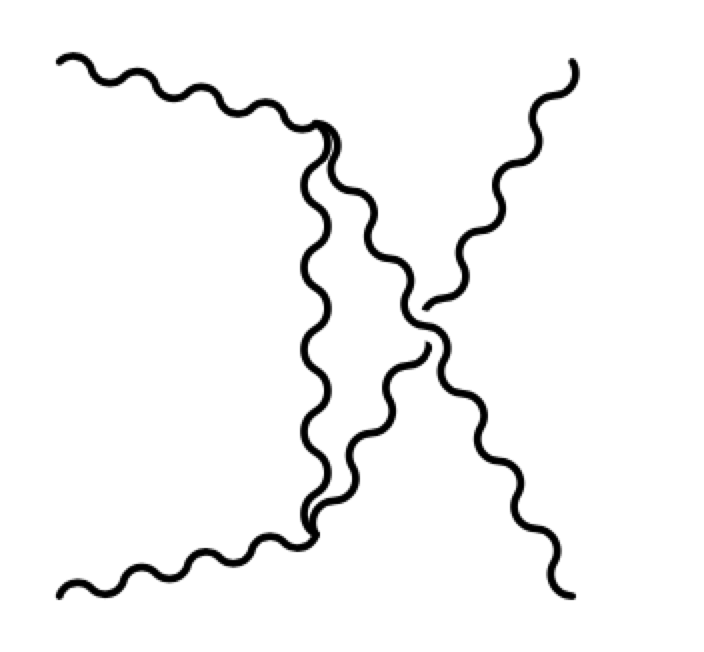
\includegraphics[width=0.21\textwidth,keepaspectratio]{figures/VBS4}
}
\caption{
The VV to VV interaction Feynman diagram at tree-level. Contributions from EW gauge boson interactions.
}
\label{fig:VBSEW}
\end{center}
\end{figure}

\begin{figure}[tbp]
\begin{center}
\subfigure{
 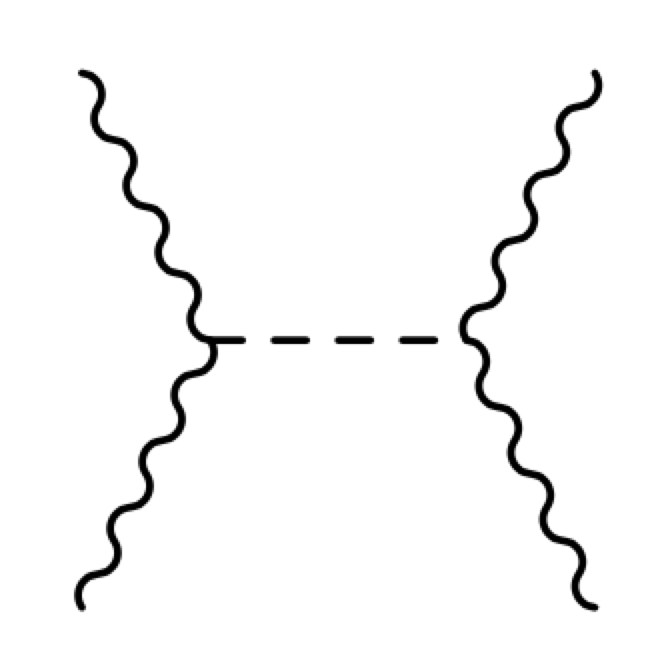
\includegraphics[width=0.20\textwidth,keepaspectratio]{figures/wHiggs1}
}
\subfigure{
 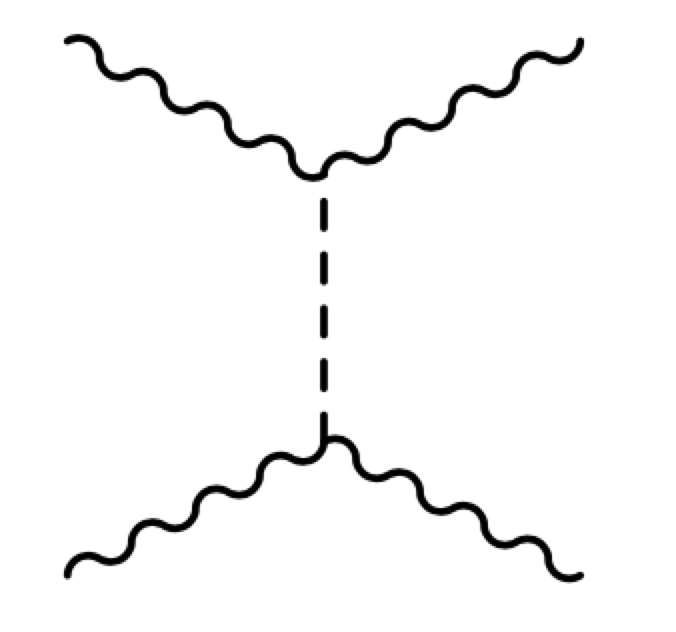
\includegraphics[width=0.20\textwidth,keepaspectratio]{figures/wHiggs2}
}
\subfigure{
 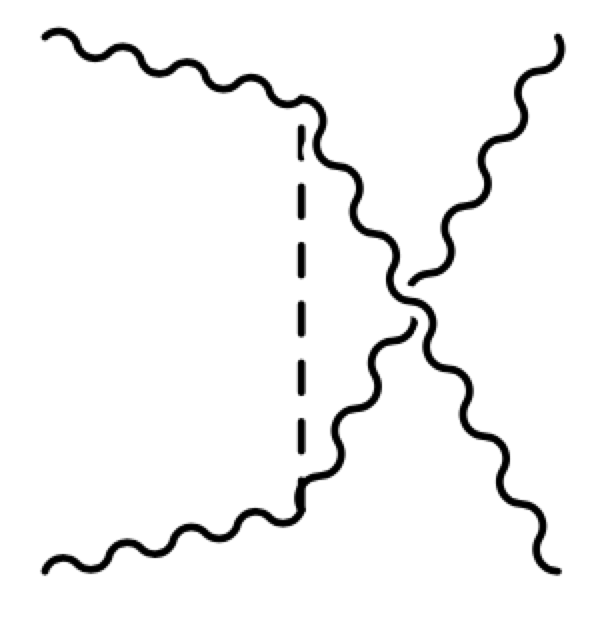
\includegraphics[width=0.18\textwidth,keepaspectratio]{figures/wHiggs3}
}
\caption{
The VV to VV interaction Feynman diagram at tree-level. Contributions includes Higgs Boson interactions.
}
\label{fig:VBSHiggs}
\end{center}
\end{figure}


The amplitude of the WW scattering is to be inspected further to see the effect of existence of the Higgs boson for example. The combination of other weak massive bosons like WZ, as well as ZZ can be denoted similarly. 
%really?

Since the polarization vector of the longitudinal weak vector boson can be written in the form, \ref{}: %put reference!
\begin{equation}
\epsilon_{L}^{\mu}=\frac{1}{m_{V}}\left(|\vec{p}|, \frac{\vec{p}}{|\vec{p}|} E\right)=\frac{p^{\mu}}{m_{V}}+\mathcal{O}\left(\frac{m_{V}}{E}\right)
\end{equation}
as the pT glows, the yields with massive vector particles in the initial and finals states will be longitudinal-dominant.
At high-energy limit, the amplitude for $W_L^+W_L^-$ without existing of the Higgs boson (Figure\ref{fig:VBSEW}) can be describes in the form of:
\begin{equation}
\mathcal{M}^{\text {gauge}}=-\frac{g_{w}^{2}}{4 m_{W}^{2}} u+\mathcal{O}\left(\left[\frac{E}{m_{W}}\right]^{0}\right)
\end{equation}
The remaining amplitude from the second term will rise with energy then it violates the unitarity at the unitarity bound. The amplitude including the Higgs contributions (Figure\ref{fig:VBSHiggs}) is:
\begin{equation}
\begin{aligned}
\mathcal{M}^{\text {Higgs}} &=-\frac{g^{2}}{4 m_{W}^{2}}\left[\frac{\left(s-m_{W}^{2}\right)^{2}}{s-m_{H}^{2}}+\frac{\left(t-m_{W}^{2}\right)^{2}}{t-m_{H}^{2}}\right] \\
& \approx \frac{g^{2}}{4 m_{W}^{2}} u,
\end{aligned}
\end{equation}
in the high-energy limit s >> $m_{H}^{2}$, $m_{W}^{2}$.
Therefore the terms affected by the rising energy cancel and leave the constant term, which is not violating the unitarity.
%The energy scale where the unitarity is violated

This effect also described with the Figure~\ref{fig:violation}.
The figure shows that if diagrams with Higgs contribution is missing, the electroweak couplings becomes strong around $\sqrt{s}$ ∼ 1 TeV, and the unitarity of the $W_LW_L \rightarrow W_LW_L$ process is violated, which means the SM without the Higgs boson is no longer valid above TeV-scale. 

\begin{figure}[tbp]
\begin{center}
%\subfigure[]{
 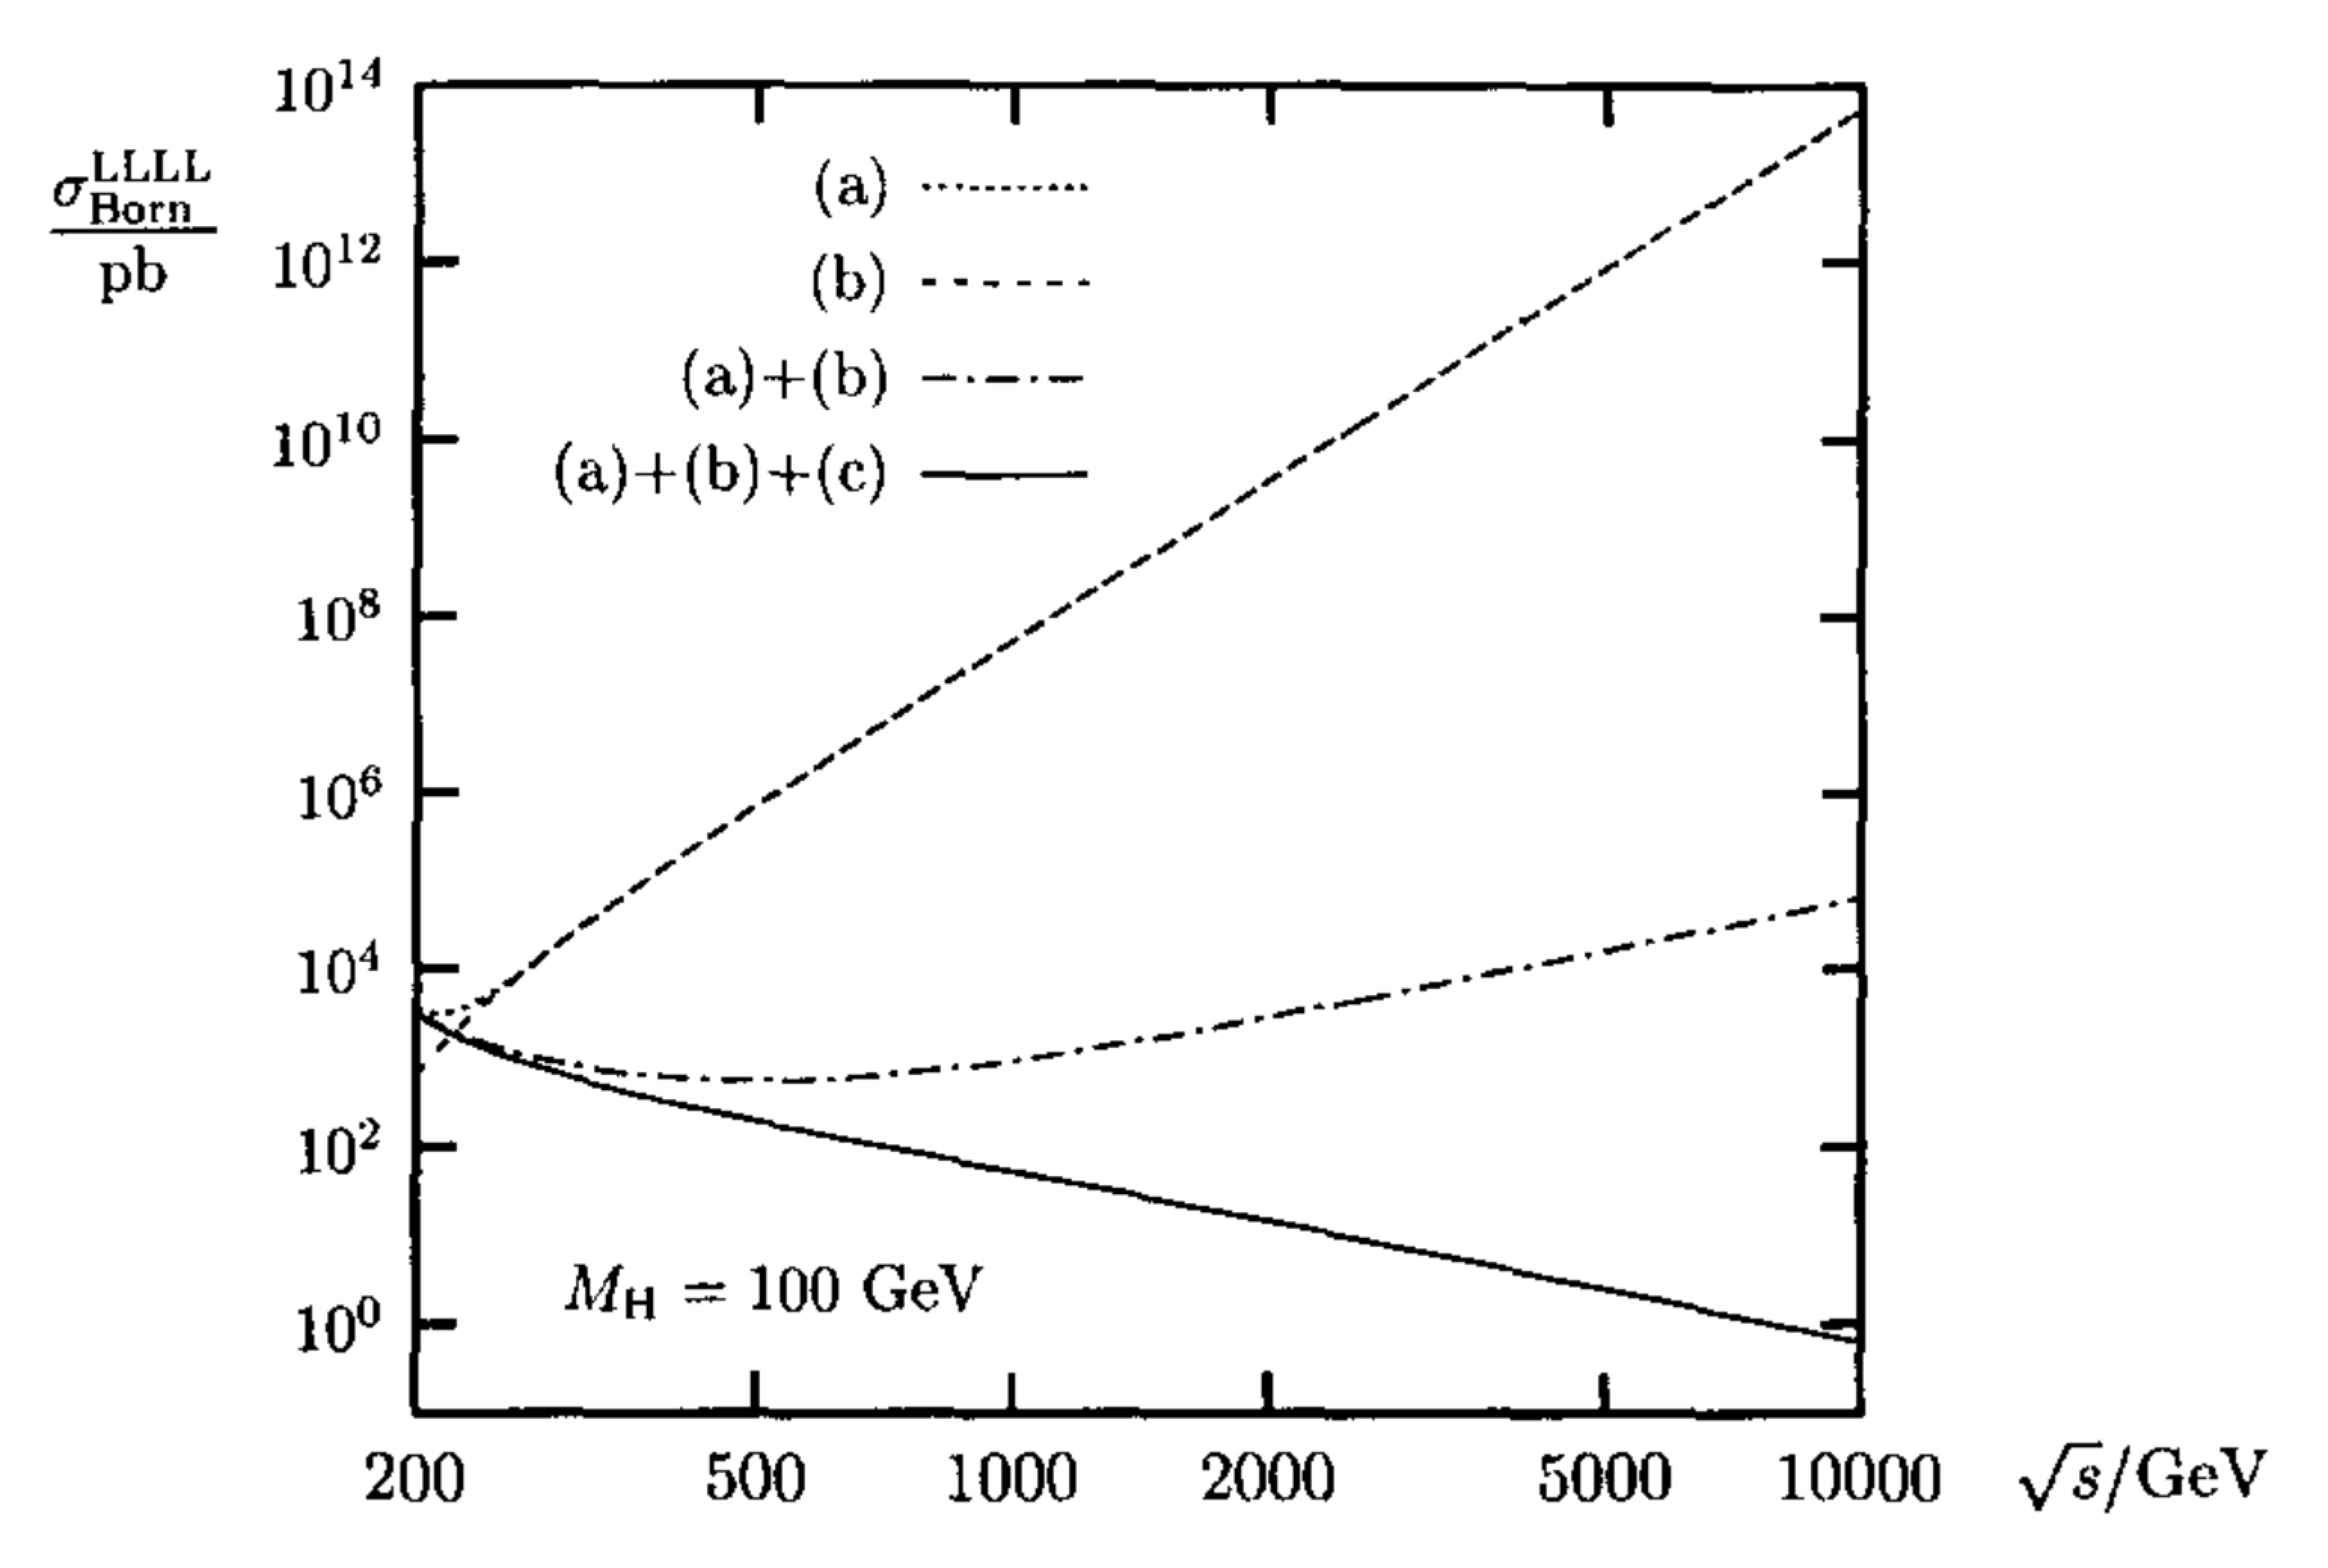
\includegraphics[width=0.80\textwidth,keepaspectratio]{figures/violation}
%}
\caption{
Cross section at tree-level %\ref{}
}
\label{fig:violation}
\end{center}
\end{figure}

\section{Production Cross-Sections and Branching Fractions}
\\
\\

\section{Anomalous Quartic Gauge Coupling and Effective Field Theory}

\subsection{aQGC}
The unitarity recovered by the existence of Higgs boson can be broken again by the additional quartic gauge coupling by new physics. This is referred to as anomalous quartic gauge couplings (aQGC). 

\subsection{EFT}
Since the aQGC can claim many different models, The Effective Field Theory (EFT) is considered as a model-independent way of the interpretation. The EFT models the effects of new physics at energy scale much higher than the currently accessible range by the experiments. The SM is a effective theory at low-energy in this framework.The EFT contains additional operators with higher energy dimension suppressed by the cutoff scale of the new physics, $\Lambda$.
The EFT Lagrangian is given as:
\begin{equation}
\mathcal{L}_{\mathrm{EFT}}=\mathcal{L}_{\mathrm{SM}}+\sum_{d>4} \sum_{i} \frac{c_{i}^{(d)}}{\Lambda^{d-4}} \mathcal{O}_{i}^{(d)}
\end{equation}
where $c_{i}^{(d)}$ are the coefficients of the new operators, $\mathcal{O}_{i}^{(d)}$.
$\Lambda$ is a cutoff scale, and the d is a mass dimension which fulfill d > 4.
Any new physics can be modeled in this framework by certain additional operators, where their coefficient is also fixed as long as the new physics scale is above the cutoff scale, $\Lambda$. The SM is a low-energy theory in this framework, i.e. if $\Lambda \rightarrow \infty$, the SM is reproduced.
\\

To model possible aQGC effect in the VBS process, the Eboli model \cite{eboli2006p} which introduces new dimension 8 operators which satisfy the SM $SU(2)\times U(1)_Y$ symmetry is used. 

The lowest dimension operator that leads to quartic interactions and does not exhibit two or three weak gauge boson vertices is dimension 8. 
This is when we get a weak boson field either from the covariant derivative of Higgs doublet $\Phi$ or from the field strength tensor. 
In either case the vector field is accompanied by a vacuum expected value or a derivative, therefore the genuine quartic vertices are of dimension 8 or higher.
%understand this?
All the corresponding operators are shown hereafter.

\begin{itemize}
\item Operators containing just $D_\mu \Phi$
\begin{equation}
\begin{aligned}
\mathcal{L}_{S, 0} &=\left[\left(D_{\mu} \Phi\right)^{\dagger} D_{\nu} \Phi\right] \times\left[\left(D^{\mu} \Phi\right)^{\dagger} D^{\nu} \Phi\right] \\
\mathcal{L}_{S, 1} &=\left[\left(D_{\mu} \Phi\right)^{\dagger} D^{\mu} \Phi\right] \times\left[\left(D_{\nu} \Phi\right)^{\dagger} D^{\nu} \Phi\right] \\
\mathcal{L}_{S, 2} &=\left[\left(D_{\mu} \Phi\right)^{\dagger} D_{\nu} \Phi\right] \times\left[\left(D^{\nu} \Phi\right)^{\dagger} D^{\mu} \Phi\right]
\end{aligned}
\end{equation}
\item Operators containing $D_\mu \Phi$ and field strength 
\begin{equation}
\begin{aligned}
\mathcal{L}_{M, 0} &=\operatorname{Tr}\left[\hat{W}_{\mu \nu} \hat{W}^{\mu \nu}\right] \times\left[\left(D_{\beta} \Phi\right)^{\dagger} D^{\beta} \Phi\right] \\
\mathcal{L}_{M, 1} &=\operatorname{Tr}\left[\hat{W}_{\mu \nu} \hat{W}^{\nu \beta}\right] \times\left[\left(D_{\beta} \Phi\right)^{\dagger} D^{\mu} \Phi\right] \\
\mathcal{L}_{M, 2} &=\left[B_{\mu \nu} B^{\mu \nu}\right] \times\left[\left(D_{\beta} \Phi\right)^{\dagger} D^{\beta} \Phi\right] \\
\mathcal{L}_{M, 3} &=\left[B_{\mu \nu} B^{\nu \beta}\right] \times\left[\left(D_{\beta} \Phi\right)^{\dagger} D^{\mu} \Phi\right] \\
\mathcal{L}_{M, 4} &=\left[\left(D_{\mu} \Phi\right)^{\dagger} \hat{W}_{\beta \nu} D^{\mu} \Phi\right] \times B^{\beta \nu} \\
\mathcal{L}_{M, 5} &=\left[\left(D_{\mu} \Phi\right)^{\dagger} \hat{W}_{\beta \nu} D^{\nu} \Phi\right] \times B^{\beta \mu} \\
\mathcal{L}_{M, 6} &=\left[\left(D_{\mu} \Phi\right)^{\dagger} \hat{W}_{\beta \nu} \hat{W}^{\beta \nu} D^{\mu} \Phi\right] \\
\mathcal{L}_{M, 7} &=\left[\left(D_{\mu} \Phi\right)^{\dagger} \hat{W}_{\beta \nu} \hat{W}^{\beta \mu} D^{\nu} \Phi\right]
\end{aligned}
\end{equation}
\item Operators containing just the field strength tensor
\begin{equation}
\begin{aligned}
\mathcal{L}_{T, 0} &=\operatorname{Tr}\left[\hat{W}_{\mu \nu} \hat{W}^{\mu \nu}\right] \times \operatorname{Tr}\left[\hat{W}_{\alpha \beta} \hat{W}^{\alpha \beta}\right] \\
\mathcal{L}_{T, 1} &=\operatorname{Tr}\left[\hat{W}_{\alpha \nu} \hat{W}^{\mu \beta}\right] \times \operatorname{Tr}\left[\hat{W}_{\mu \beta} \hat{W}^{\alpha \nu}\right] \\
\mathcal{L}_{T, 2} &=\operatorname{Tr}\left[\hat{W}_{\alpha \mu} \hat{W}^{\mu \beta}\right] \times \operatorname{Tr}\left[\hat{W}_{\beta \nu} \hat{W}^{\nu \alpha}\right] \\
\mathcal{L}_{T, 3} &=\operatorname{Tr}\left[\hat{W}_{\alpha \mu} \hat{W}^{\mu \beta} \hat{W}^{\nu \alpha}\right] \times B_{\beta \nu} \\
\mathcal{L}_{T, 4} &=\operatorname{Tr}\left[\hat{W}_{\alpha \mu} \hat{W}^{\alpha \mu} \hat{W}^{\beta \nu}\right] \times B_{\beta \nu} \\
\mathcal{L}_{T, 5} &=\operatorname{Tr}\left[\hat{W}_{\mu \nu} \hat{W}^{\mu \nu}\right] \times B_{\alpha \beta} B^{\alpha \beta} \\
\mathcal{L}_{T, 6} &=\operatorname{Tr}\left[\hat{W}_{\alpha \nu} \hat{W}^{\mu \beta}\right] \times B_{\mu \beta} B^{\alpha \nu} \\
\mathcal{L}_{T, 7} &=\operatorname{Tr}\left[\hat{W}_{\alpha \mu} \hat{W}^{\mu \beta}\right] \times B_{\beta \nu} B^{\nu \alpha} \\
\mathcal{L}_{T, 8} &=B_{\mu \nu} B^{\mu \nu} B_{\alpha \beta} B^{\alpha \beta} \\
\mathcal{L}_{T, 9} &=B_{\alpha \mu} B^{\mu \beta} B_{\beta \nu} B^{\nu \alpha}
\end{aligned}
\end{equation}
\end{itemize}

Since the operator $\mathcal{L}_{S, 2}$ is the Hermite conjugate of the $\mathcal{L}_{S, 0}$, those 2 operators are treated as single operator denoted as $\mathcal{L}_{S, 02}$, with the coefficient $f_S02$, respectively. It is found via simulations that the tensor operators produce purely transversely polarized $W/Z$ bosons, while the scalar operators longitudinal bosons.

The summary of the correspondences of the operators and the vertices are summarized in the table~\ref{tab:vertex}.

%table1
\begin{center}
\begin{tabular}{|l| c c c c c c c c c|} 
 \hline
 operators                                                & $WWWW$ & $WWZZ$ & $ZZZZ$ & $WW\gamma Z$ & $WW\gamma \gamma$ & $ZZZ\gamma$ & $ZZ\gamma \gamma$ & $Z\gamma \gamma \gamma$ & $\gamma \gamma \gamma \gamma \gamma$\\ [0.5ex] 
 \hline\hline
 $\mathcal{L}_{S02}$,$\mathcal{L}_{S1}$                   & \checkmark & \checkmark & \checkmark &  &  &  &  & & \\ 
 \hline
 $\mathcal{L}_{M0}$,$\mathcal{L}_{M1}$,$\mathcal{L}_{M7}$ & \checkmark & \checkmark & \checkmark & \checkmark & \checkmark &\checkmark &\checkmark & &\\
 \hline
 $\mathcal{L}_{M2}$,$\mathcal{L}_{M3}$,$\mathcal{L}_{M4}$,$\mathcal{L}_{M5}$ &  & \checkmark & \checkmark & \checkmark & \checkmark & \checkmark &\checkmark & &\\
 \hline
 $\mathcal{L}_{T0}$,$\mathcal{L}_{T1}$,$\mathcal{L}_{T2}$ &  & \checkmark & \checkmark & \checkmark & \checkmark & \checkmark & \checkmark & &\\
 \hline
 $\mathcal{L}_{T5}$,$\mathcal{L}_{T6}$,$\mathcal{L}_{T7}$ & \checkmark & \checkmark & \checkmark & \checkmark & \checkmark & \checkmark &\checkmark &\checkmark &\checkmark\\ [1ex] 
 \hline
 $\mathcal{L}_{T8}$,$\mathcal{L}_{T9}$                    &  &  & \checkmark &  &  & \checkmark &\checkmark &\checkmark &\checkmark\\ [1ex] 
 \hline
\end{tabular}
\caption{operators and the vertices}
\label{tab:vertex}
\end{center}

The aQGCs can be measured by the VBS and the triboson channels.
The summary of sensitive channel to each operator is shown in the table~\ref{tab:aQGCchannel}. \textcolor{blue}{need to think and modify this table}

%table2
\begin{center}
\begin{tabular}{|l| c c c c c c |} 
 \hline
 VVjj final state                                         & $ZZ$ & $WWZZ$ & $ZZZZ$ & $WW\gamma Z$ & $WW\gamma \gamma$ & $ZZZ\gamma$ \\ [0.5ex] 
 \hline\hline
 VVV final state                                          & $ZZZ$ & $WWZZ$ & $ZZZZ$ & $WW\gamma Z$ & $WW\gamma \gamma$ & $ZZZ\gamma$ \\ [0.5ex] 
 \hline\hline
 $\mathcal{L}_{S02}$,$\mathcal{L}_{S1}$                   & \checkmark & \checkmark & \checkmark &  &           &  \\ 
 \hline
 $\mathcal{L}_{M0}$,$\mathcal{L}_{M1}$,$\mathcal{L}_{M7}$ & \checkmark & \checkmark & \checkmark & \checkmark & \checkmark &\checkmark \\
 \hline
 $\mathcal{L}_{M2}$,$\mathcal{L}_{M3}$,$\mathcal{L}_{M4}$,$\mathcal{L}_{M5}$ &  & \checkmark & \checkmark & \checkmark & \checkmark & \checkmark\\
 \hline
 $\mathcal{L}_{T0}$,$\mathcal{L}_{T1}$,$\mathcal{L}_{T2}$ &  & \checkmark & \checkmark & \checkmark & \checkmark & \checkmark \\
 \hline
 $\mathcal{L}_{T5}$,$\mathcal{L}_{T6}$,$\mathcal{L}_{T7}$ & \checkmark & \checkmark & \checkmark & \checkmark & \checkmark & \checkmark \\ [1ex] 
 \hline
 $\mathcal{L}_{T8}$,$\mathcal{L}_{T9}$                    &  &  & \checkmark &  &  & \checkmark \\ [1ex] 
 \hline
\end{tabular}
\caption{operators and the channels}
\label{tab:aQGCchannel}
\end{center}

